\documentclass[Main]{subfiles}

\begin{document}

\chapter{Scope}

\section{Identification}
This Preliminary Design Description (PDD) identifies, specifies and establishes an overview of the system design for the Self Protection Suite (SPS).

\section{System overview}
The purpose of the SPS is to provide the Royal Danish Air Force with a self-protection suite for the F-16 combat aircraft which will dispense payloads and host a MWS. 
The system will provide warning upon detection of missile threats and automatically dispense payloads in response.

\begin{figure}[H]
\centering
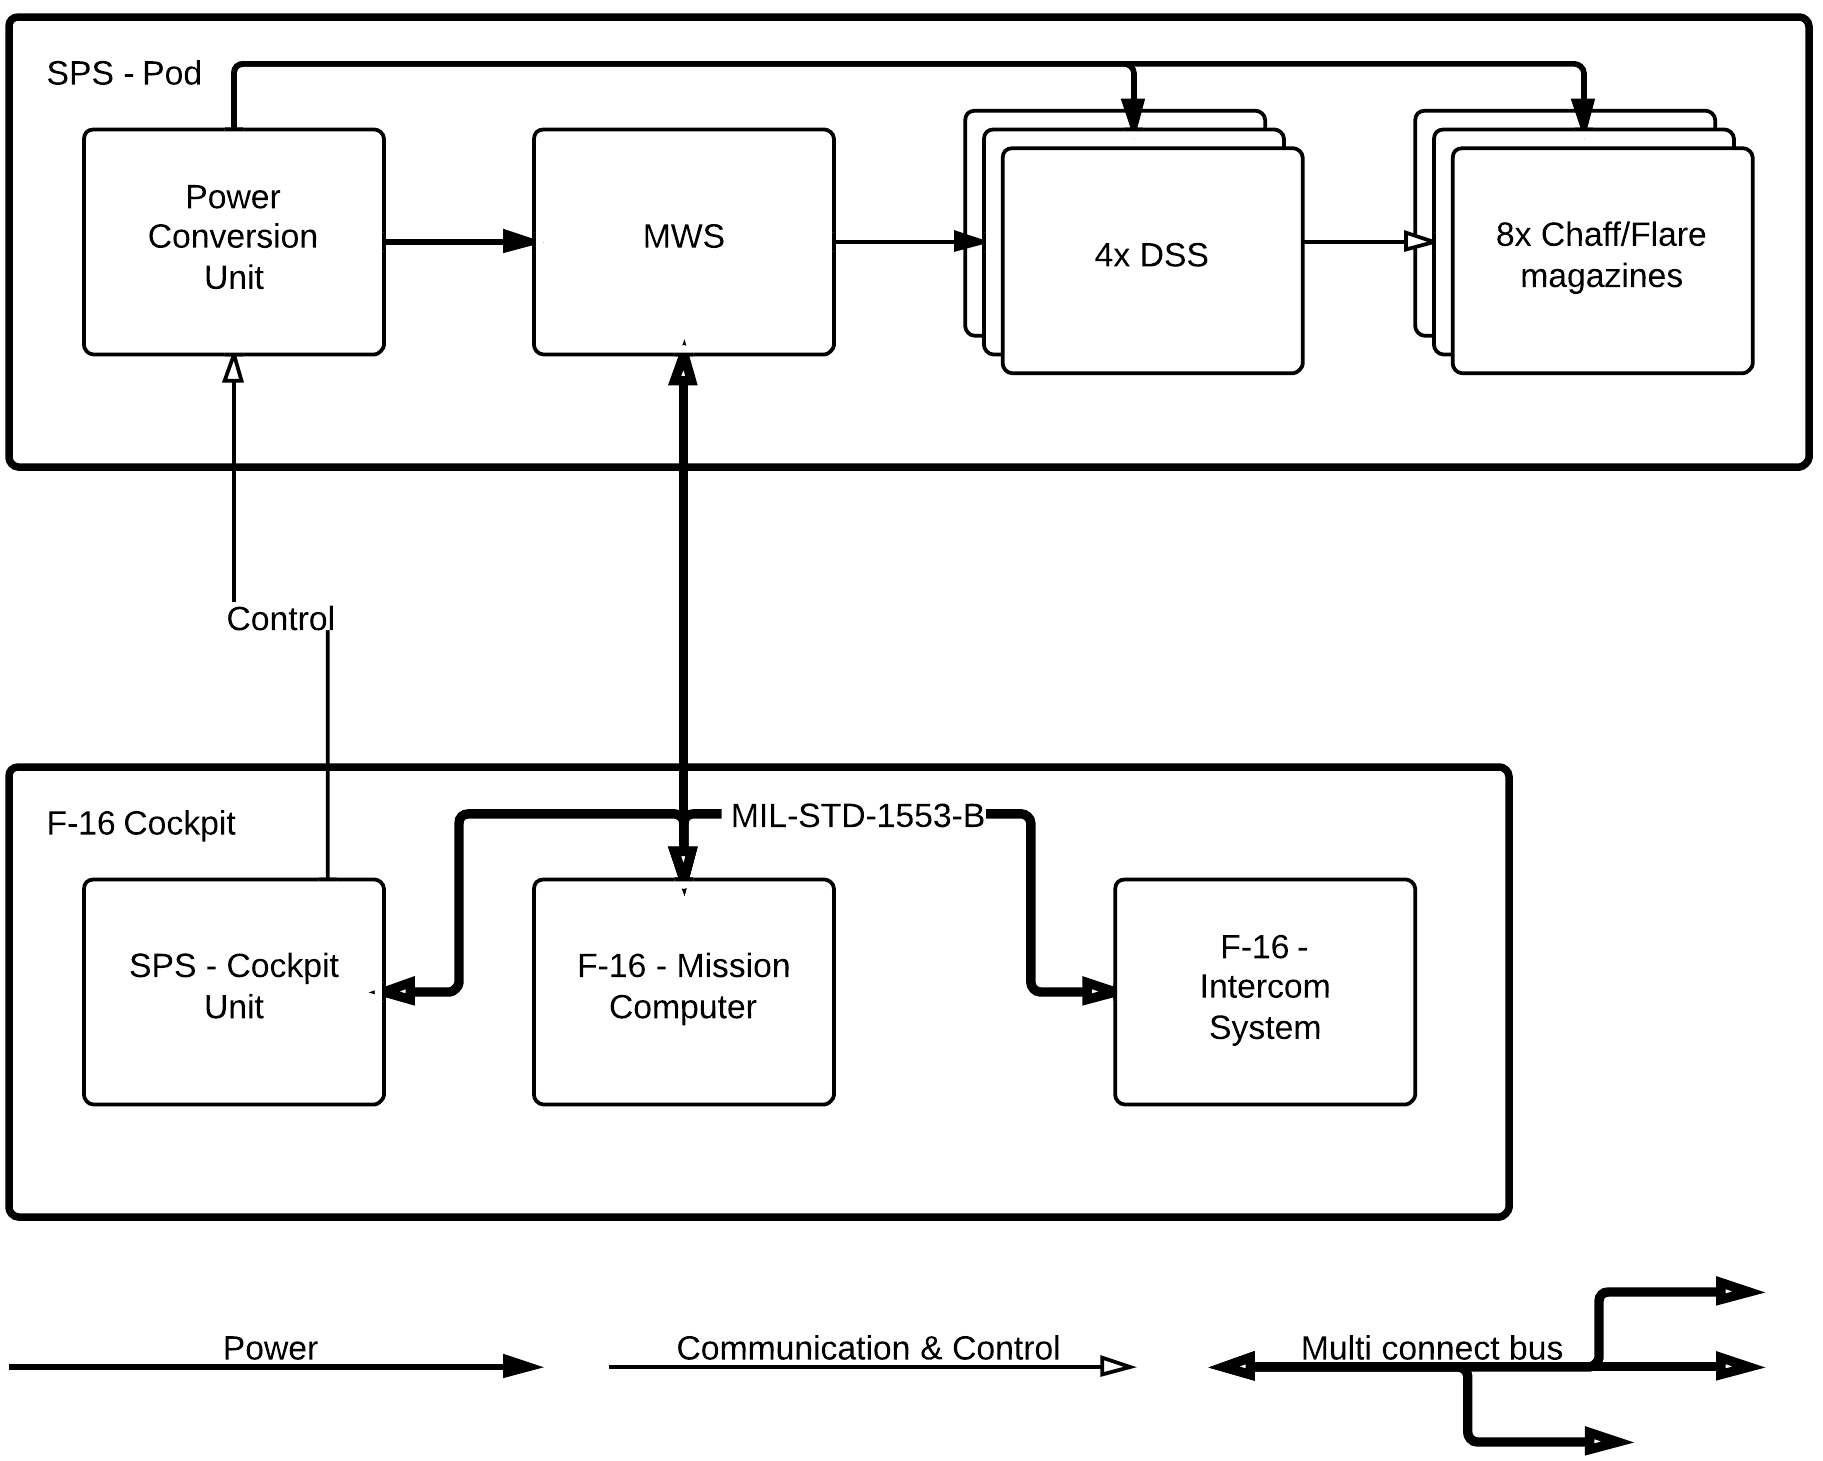
\includegraphics[width = 0.9\textwidth]{ConceptOfOperations}
\caption{Concept of operations}
\end{figure}


\section{Document overview}
This section has been tailored out. See Table of Contents.



\end{document}